% TeX eps-loader file generated by stoch_simul.m (Dynare).
% 14-Apr-2024 18:36:27
 
\begin{figure}[H]
\centering 
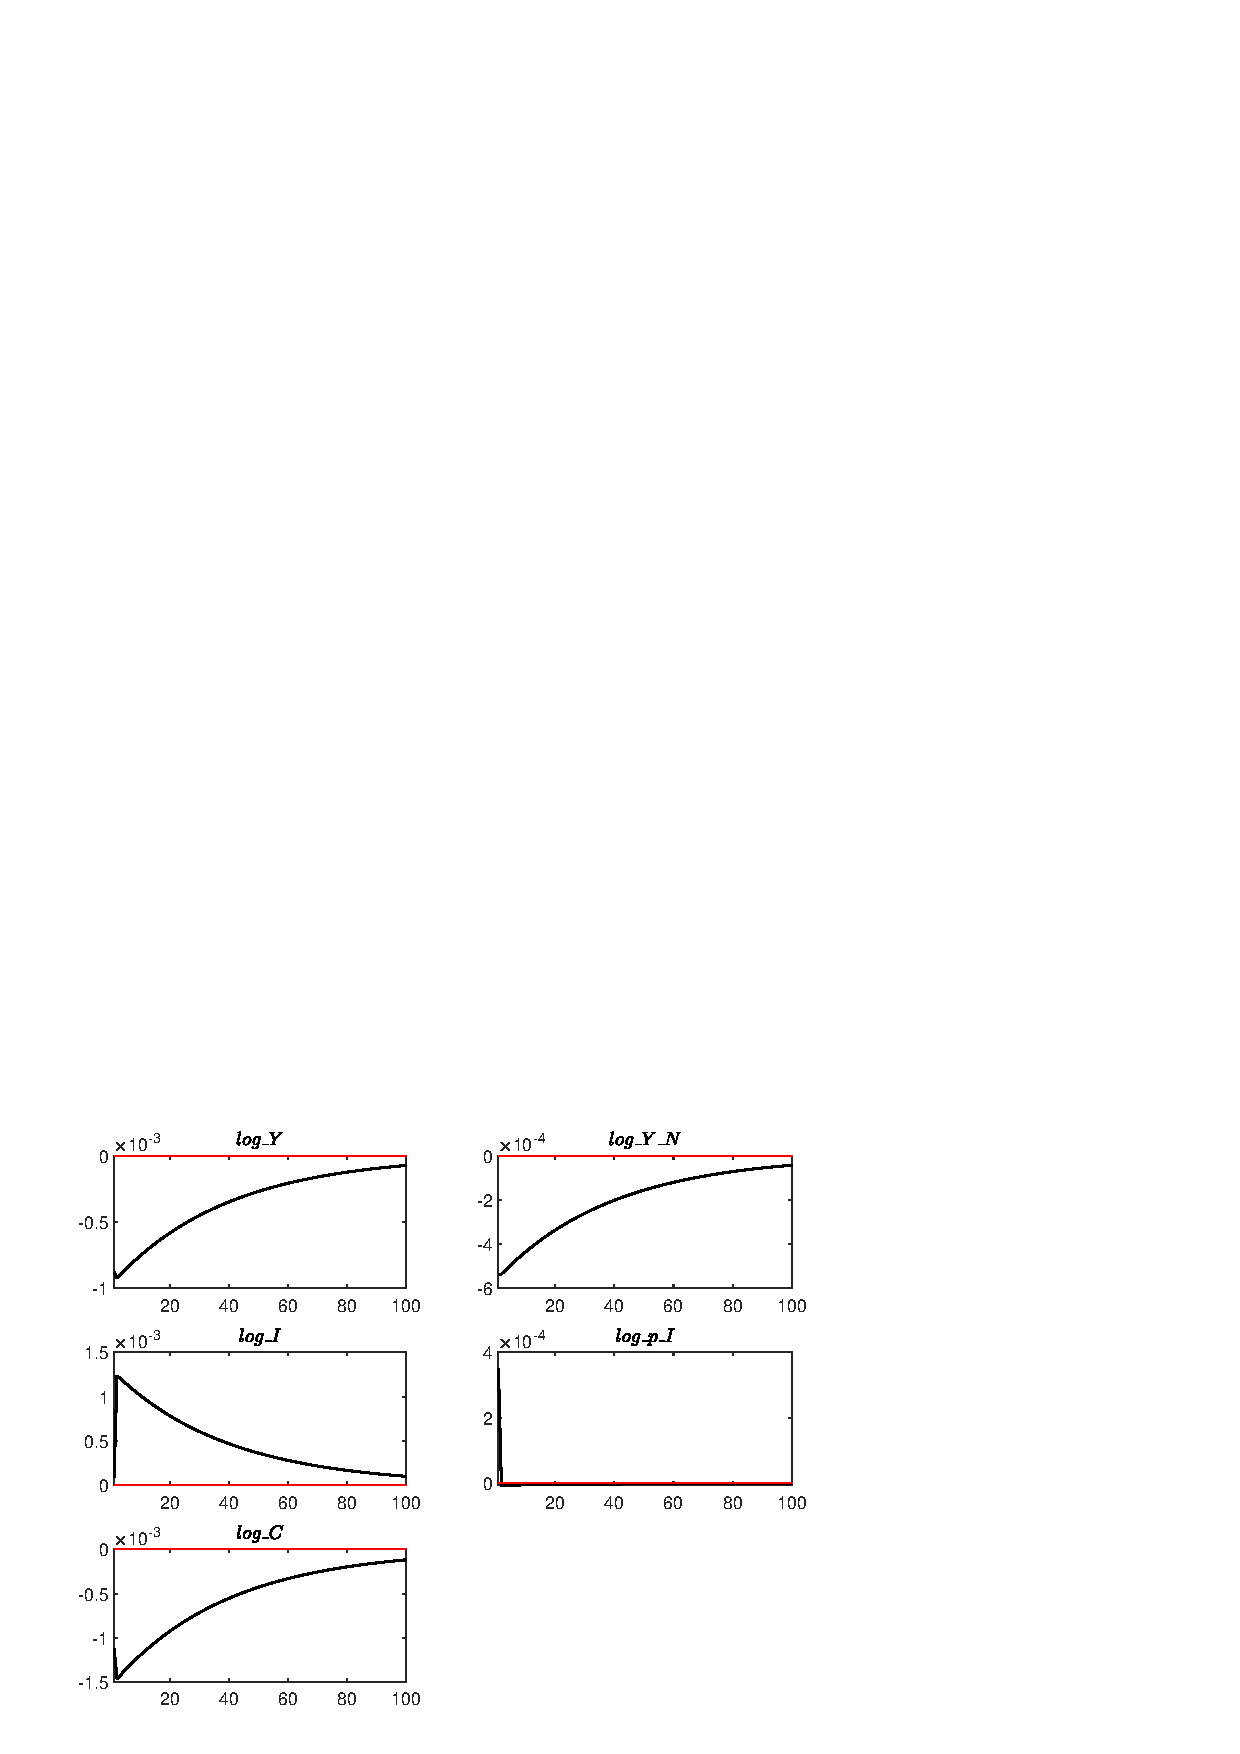
\includegraphics[width=0.80\textwidth]{BRS_growth/graphs/BRS_growth_IRF_e_g}
\caption{Impulse response functions (orthogonalized shock to ${e_g}$).}
\label{Fig:IRF:e_g}
\end{figure}
 
\begin{figure}[H]
\centering 
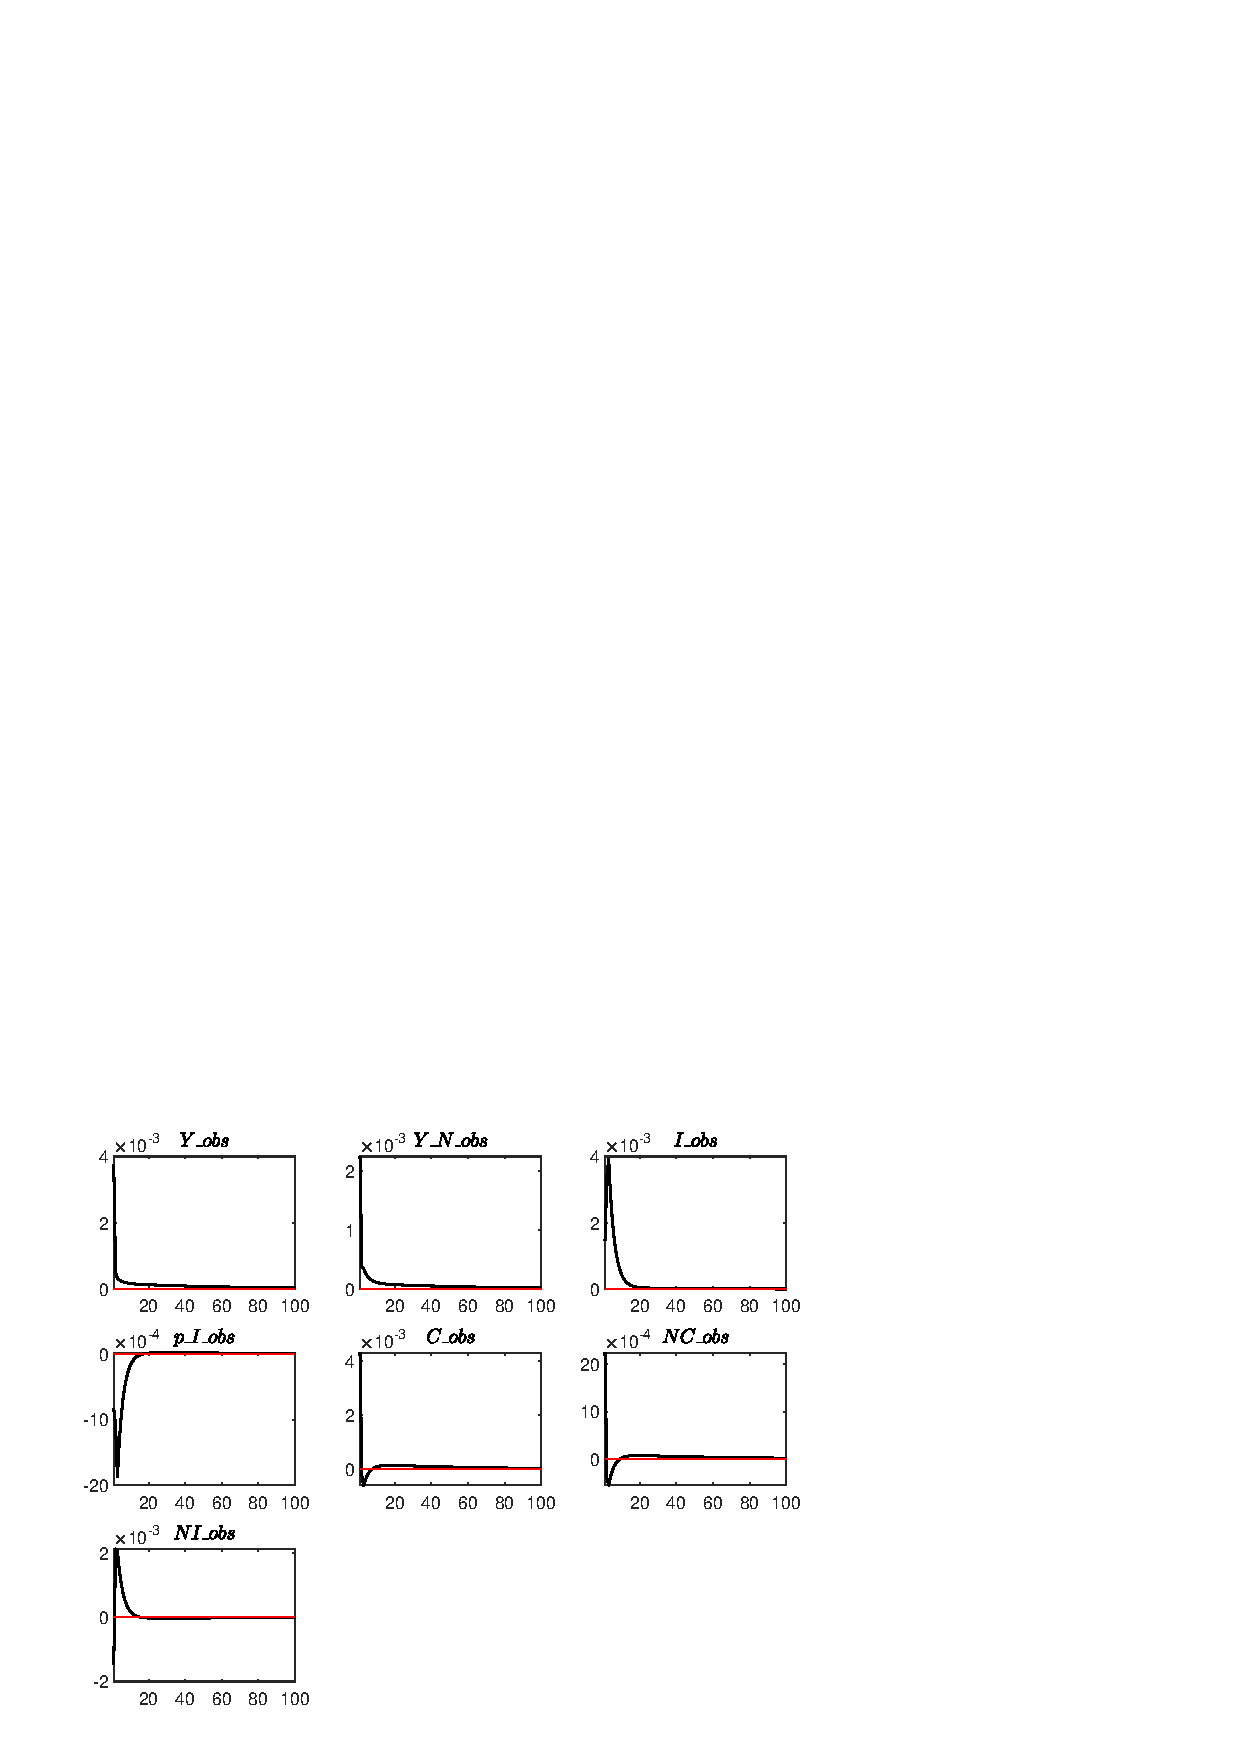
\includegraphics[width=0.80\textwidth]{BRS_growth/graphs/BRS_growth_IRF_e_Z}
\caption{Impulse response functions (orthogonalized shock to ${e_Z}$).}
\label{Fig:IRF:e_Z}
\end{figure}
 
\begin{figure}[H]
\centering 
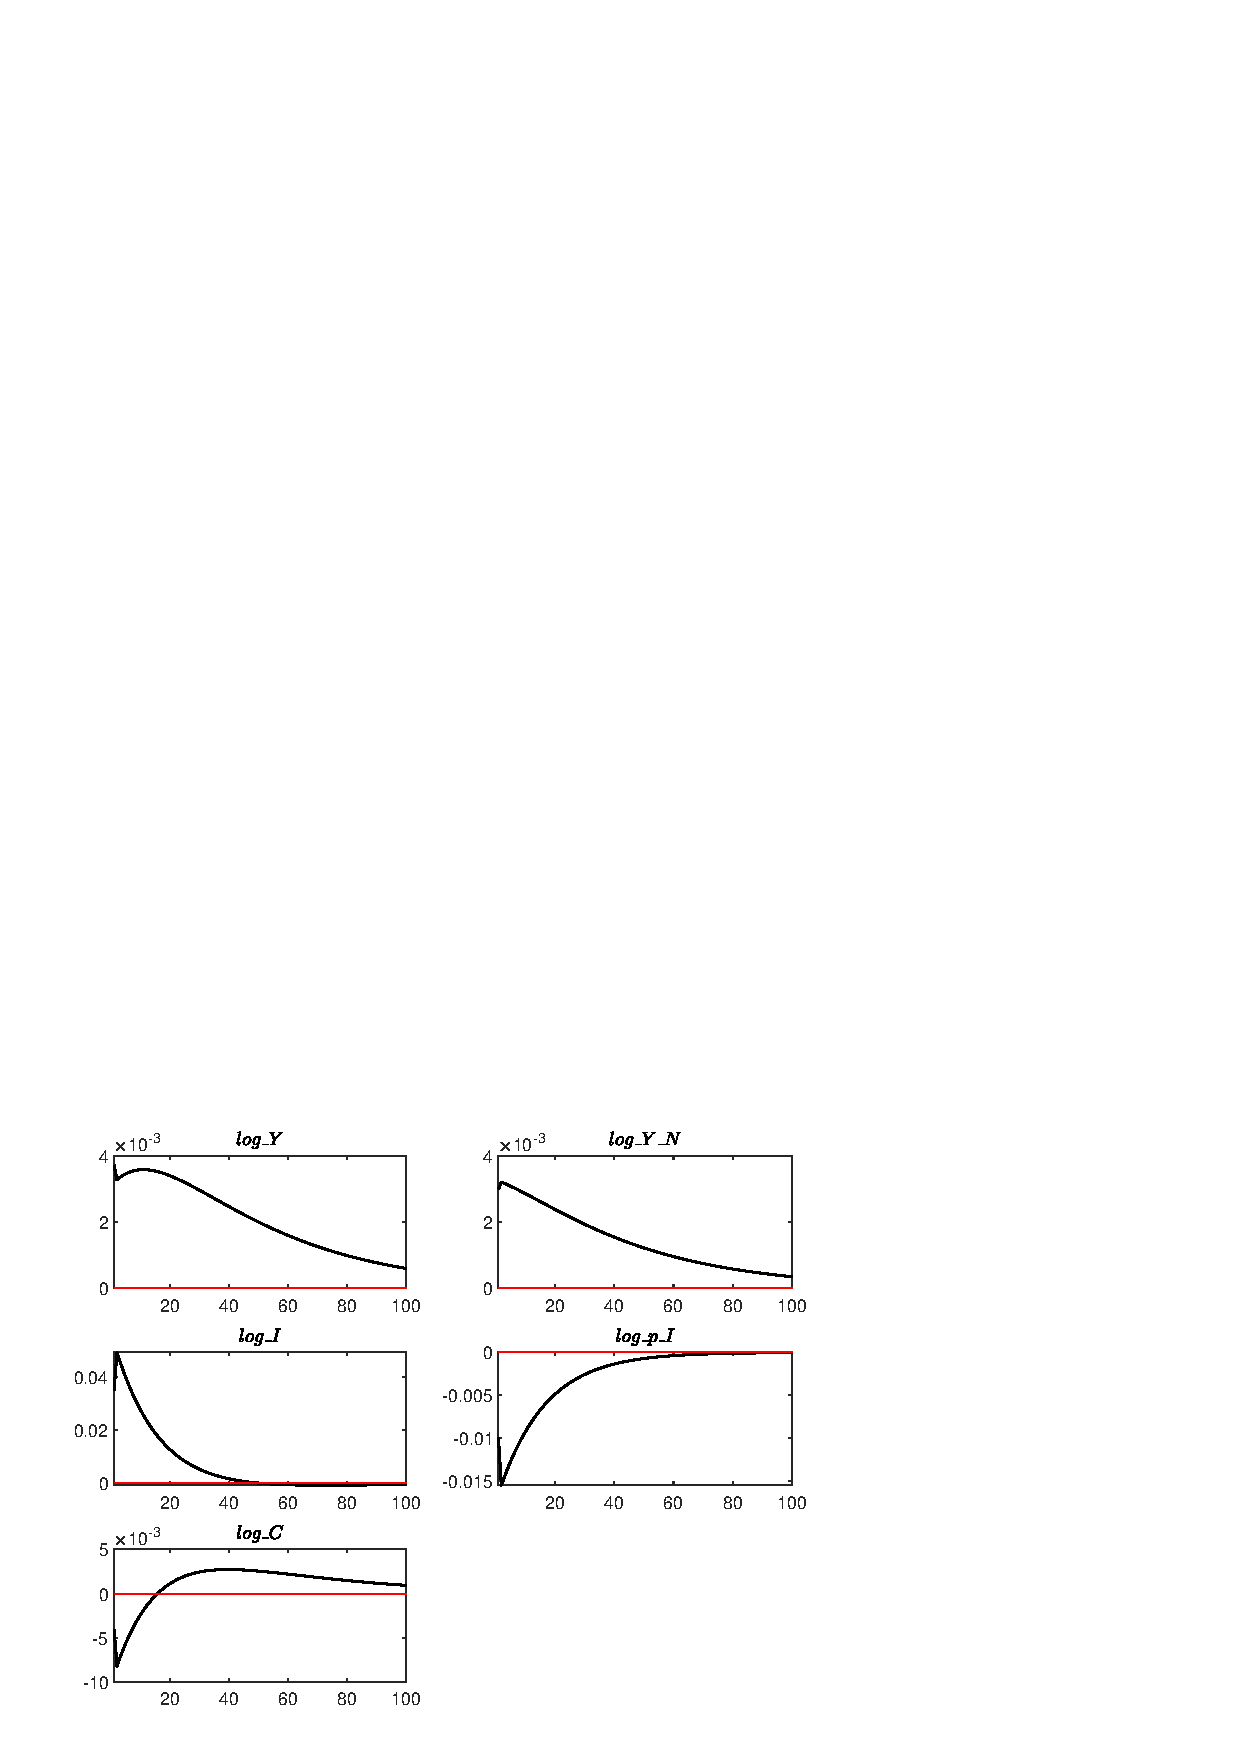
\includegraphics[width=0.80\textwidth]{BRS_growth/graphs/BRS_growth_IRF_e_ZI}
\caption{Impulse response functions (orthogonalized shock to ${e_{ZI}}$).}
\label{Fig:IRF:e_ZI}
\end{figure}
 
\begin{figure}[H]
\centering 
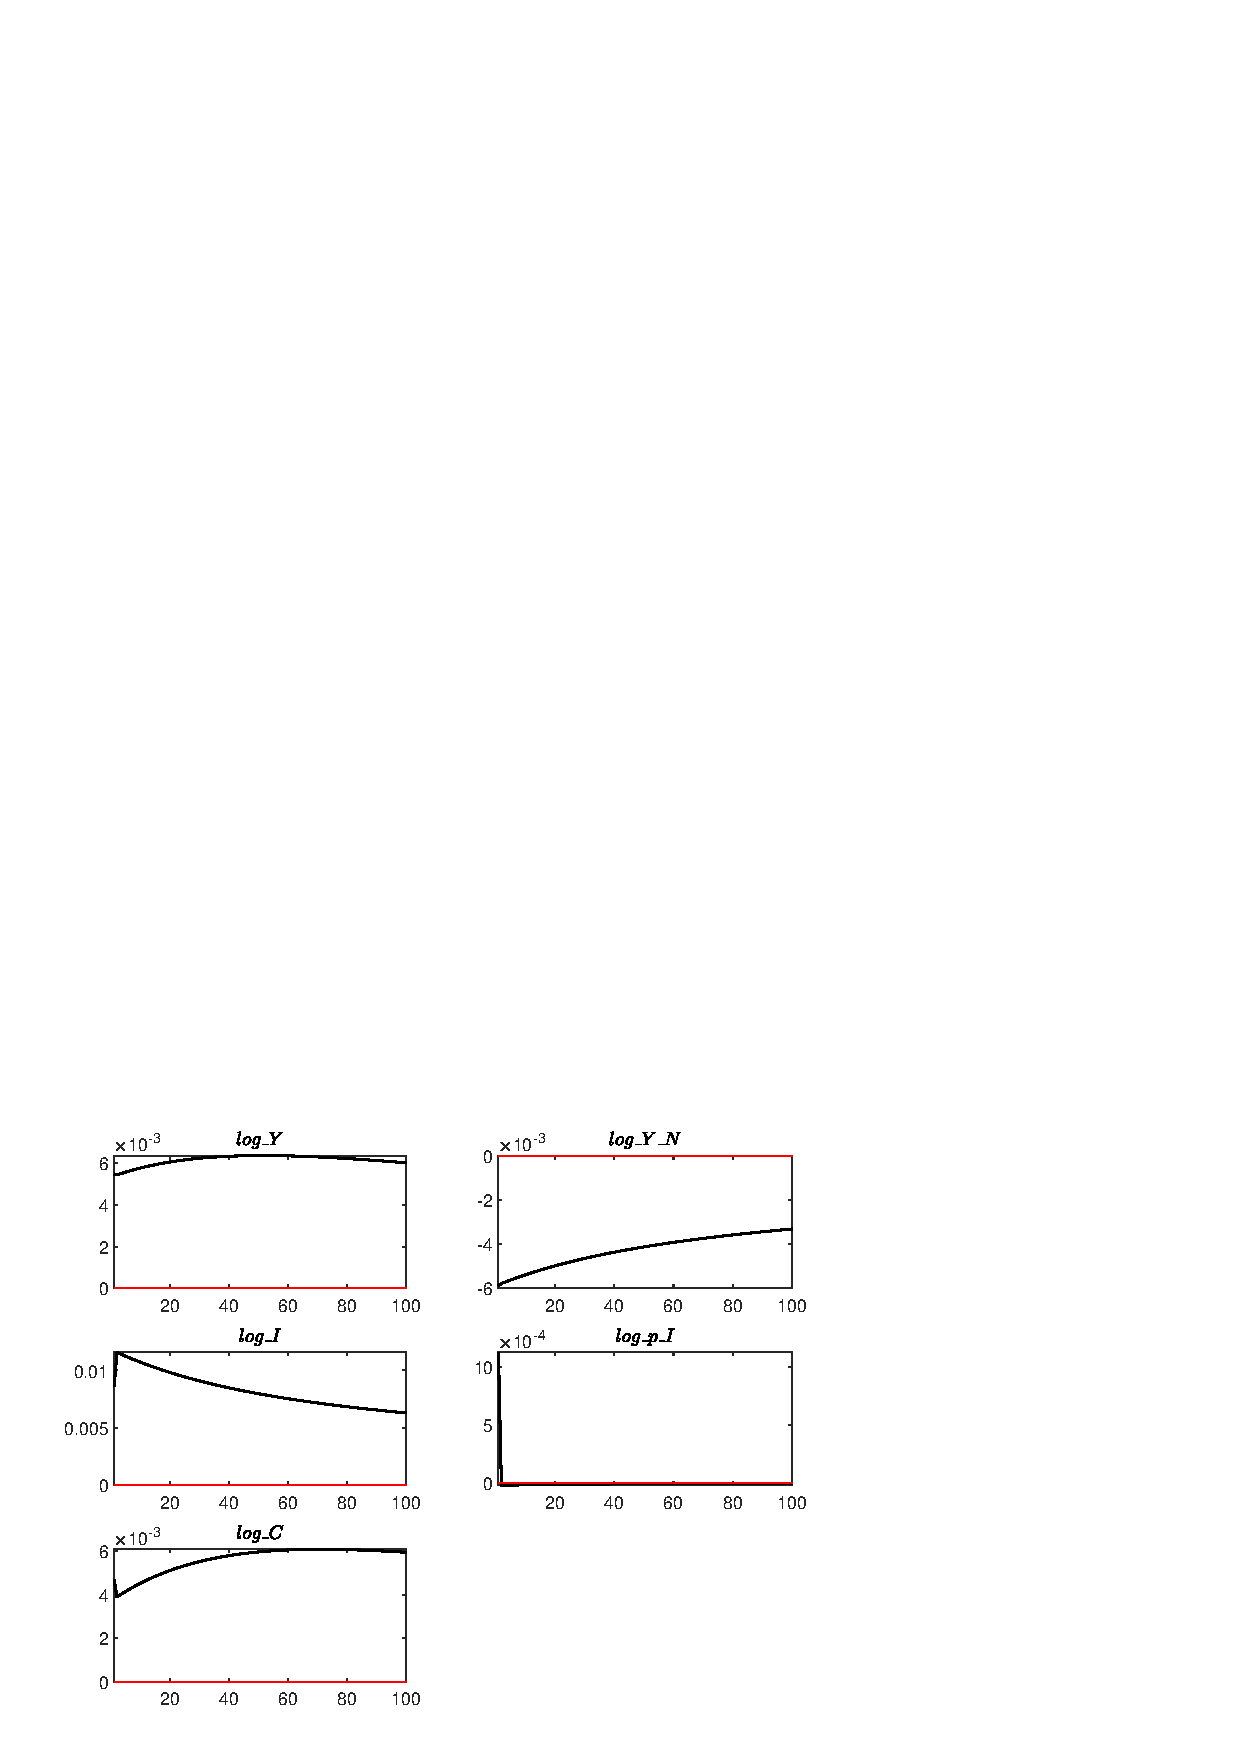
\includegraphics[width=0.80\textwidth]{BRS_growth/graphs/BRS_growth_IRF_e_N}
\caption{Impulse response functions (orthogonalized shock to ${e_N}$).}
\label{Fig:IRF:e_N}
\end{figure}
 
\begin{figure}[H]
\centering 
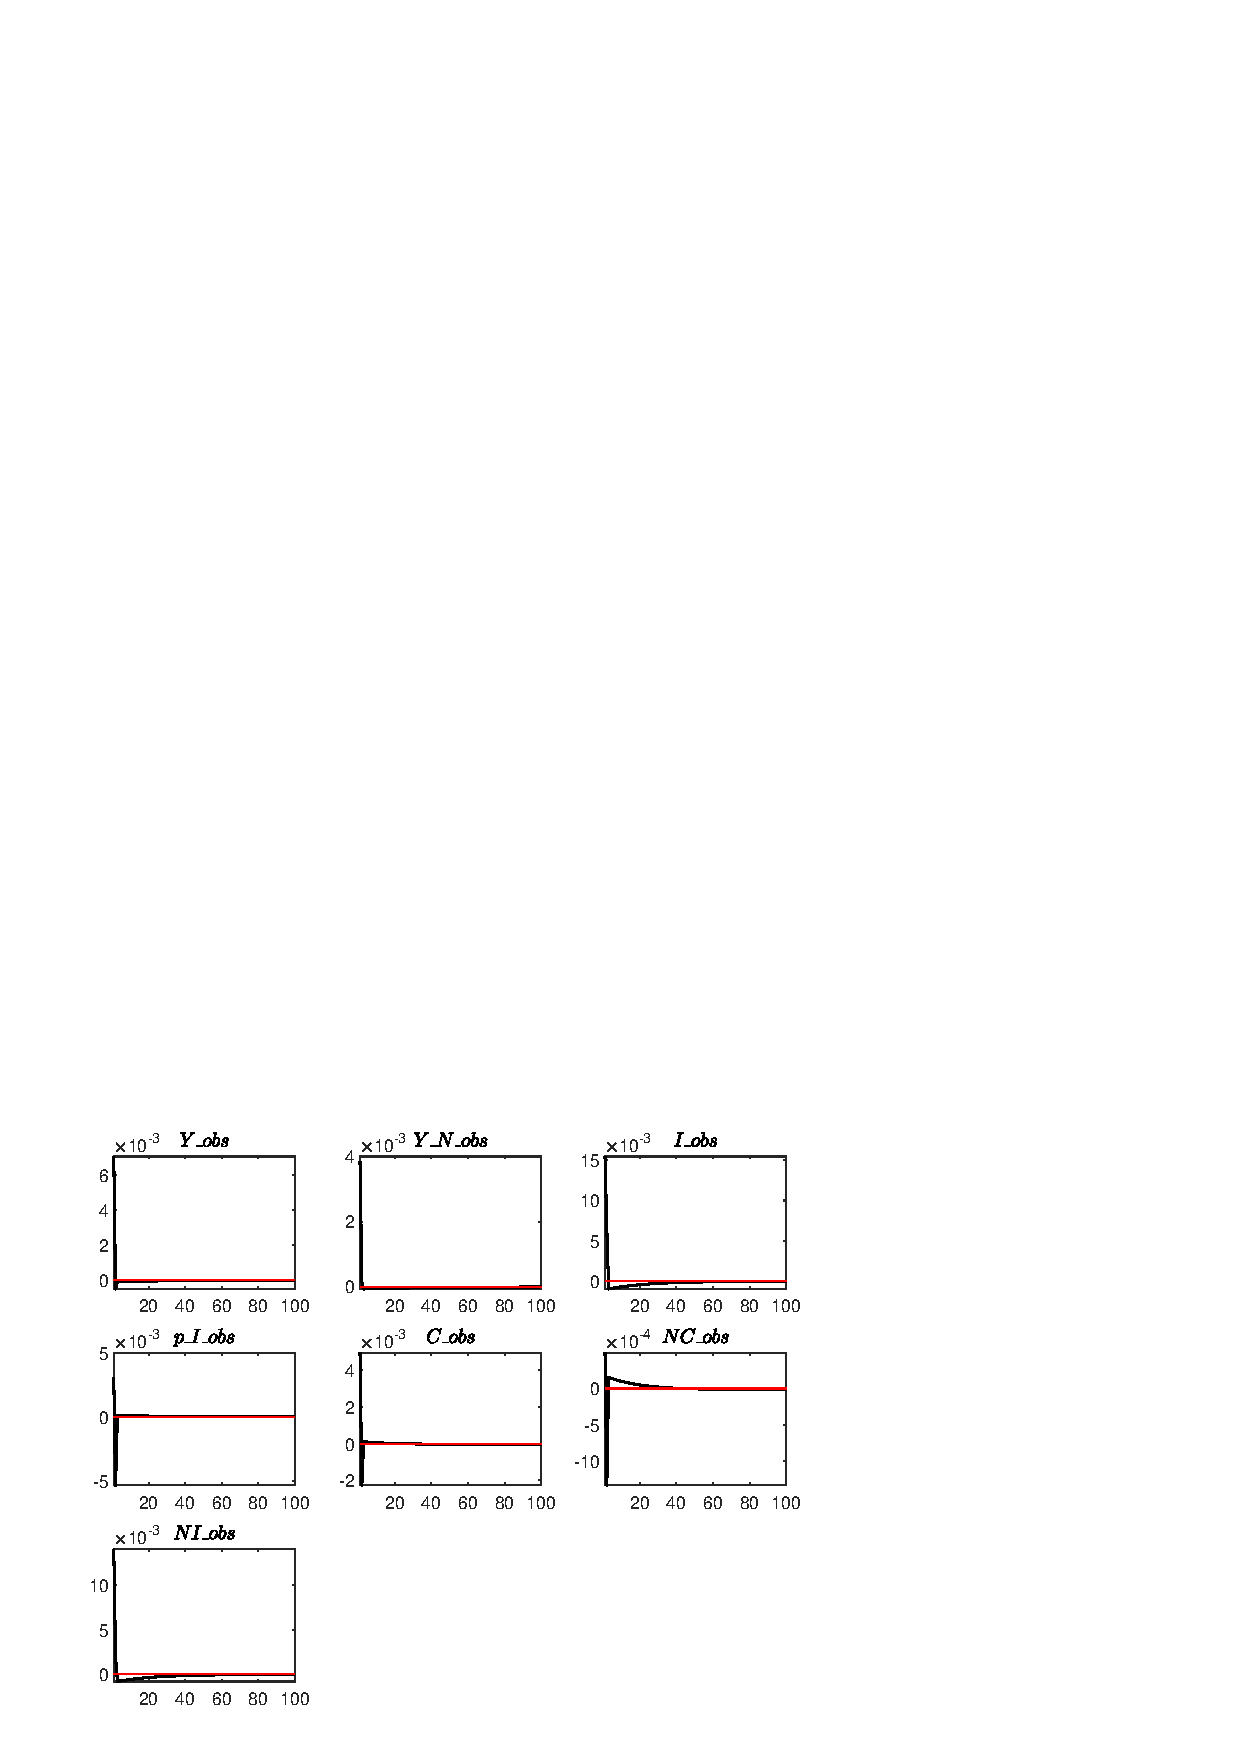
\includegraphics[width=0.80\textwidth]{BRS_growth/graphs/BRS_growth_IRF_e_D}
\caption{Impulse response functions (orthogonalized shock to ${e_D}$).}
\label{Fig:IRF:e_D}
\end{figure}
 
 
% End Of TeX file. 
